% J-Curve
% Author: Rasmus Pank Roulund
\documentclass{minimal}
\usepackage{tikz}
\usetikzlibrary{calc,arrows}
\usepackage{verbatim}

\begin{comment}
:Title: J-Curve
:Tags: Plots, Coord. calculations

An illustration of a country�s trade balance following a devaluation. The shape of the curve
is known as a J-curve_.

.. _j-curve: http://en.wikipedia.org/wiki/J_curve

:Author: Rasmus Pank Roulund

\end{comment}


\begin{document}

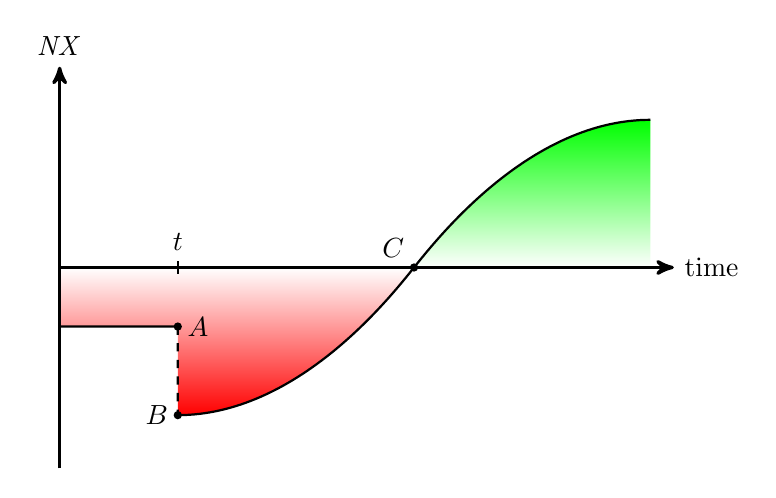
\begin{tikzpicture}[
        %We set the scale and define some styles
        scale=1.5,
        axis/.style={very thick, ->, >=stealth'},
        important line/.style={thick},
        dashed line/.style={dashed, thick},
        every node/.style={color=black,}
     ]
    % Important coordinates are defined
    \coordinate (beg_1) at (0,-.5);
    \coordinate (beg_2) at ($(beg_1)+(1,0)$);
    \coordinate (dev_1) at ($(beg_2)+(0,-.75)$);
    \coordinate (xint) at (3,0);
    \coordinate (end) at (5,1.25);

    %We make some nice shading to annotate different parts of the curve
    % Everything for x<0
    \begin{scope}
        \shade[top color=white, bottom color=red]
            ($(beg_2)+(0,.5)$) parabola bend (dev_1) (xint)
            (0,0) rectangle (beg_2);
    \end{scope}
    %  Everything for x>0
    \begin{scope}
        \shade[bottom color=white, top color=green]
            (xint) parabola bend (end) ($(end)+(0,-1.25)$);
    \end{scope}
    % axis
    \draw[axis] (0,0)  -- (5.2,0) node(xline)[right] {time};
    \draw[axis] (0,-1.7) -- (0,1.7) node(yline)[above] {$\mathit{NX}$};
    % J curve is drawn
    \draw[important line]
        (beg_1) -- (beg_2)
        (dev_1) parabola (xint)
        (xint) parabola[bend at end] (end);
    % coordinates are added
    \fill[black] (beg_2) circle (1pt) node[right] {$A$};
    \fill[black] (dev_1) circle (1pt) node[left] {$B$};
    \fill[black] (xint) circle (1pt) node[above left] {$C$};
    % The time of the devaluation is added
    \draw[dashed line] (beg_2) -- (dev_1);
    \draw[thick] (1,-1.5pt) -- (1,1.5pt) node[above] {$t$};
\end{tikzpicture}

\end{document}
